\documentclass[handout,nooutcomes,noauthor]{ximera}

\graphicspath{  
{./}
{./whoAreYou/}
{./drawingWithTheTurtle/}
{./bisectionMethod/}
{./circles/}
{./anglesAndRightTriangles/}
{./lawOfSines/}
{./lawOfCosines/}
{./plotter/}
{./staircases/}
{./pitch/}
{./qualityControl/}
{./symmetry/}
{./nGonBlock/}
}


%% page layout
\usepackage[cm,headings]{fullpage}
\raggedright
\setlength\headheight{13.6pt}


%% fonts
\usepackage{euler}

\usepackage{FiraMono}
\renewcommand\familydefault{\ttdefault} 
\usepackage[defaultmathsizes]{mathastext}
\usepackage[htt]{hyphenat}

\usepackage[T1]{fontenc}
\usepackage[scaled=1]{FiraSans}

%\usepackage{wedn}
\usepackage{pbsi} %% Answer font


\usepackage{cancel} %% strike through in pitch/pitch.tex


%% \usepackage{ulem} %% 
%% \renewcommand{\ULthickness}{2pt}% changes underline thickness

\tikzset{>=stealth}

\usepackage{adjustbox}

\setcounter{titlenumber}{-1}

%% journal style
\makeatletter
\newcommand\journalstyle{%
  \def\activitystyle{activity-chapter}
  \def\maketitle{%
    \addtocounter{titlenumber}{1}%
                {\flushleft\small\sffamily\bfseries\@pretitle\par\vspace{-1.5em}}%
                {\flushleft\LARGE\sffamily\bfseries\thetitlenumber\hspace{1em}\@title \par }%
                {\vskip .6em\noindent\textit\theabstract\setcounter{question}{0}\setcounter{sectiontitlenumber}{0}}%
                    \par\vspace{2em}
                    \phantomsection\addcontentsline{toc}{section}{\thetitlenumber\hspace{1em}\textbf{\@title}}%
                     }}
\makeatother



%% thm like environments
\let\question\relax
\let\endquestion\relax

\newtheoremstyle{QuestionStyle}{\topsep}{\topsep}%%% space between body and thm
		{}                      %%% Thm body font
		{}                              %%% Indent amount (empty = no indent)
		{\bfseries}            %%% Thm head font
		{)}                              %%% Punctuation after thm head
		{ }                           %%% Space after thm head
		{\thmnumber{#2}\thmnote{ \bfseries(#3)}}%%% Thm head spec
\theoremstyle{QuestionStyle}
\newtheorem{question}{}



\let\freeResponse\relax
\let\endfreeResponse\relax

%% \newtheoremstyle{ResponseStyle}{\topsep}{\topsep}%%% space between body and thm
%% 		{\wedn\bfseries}                      %%% Thm body font
%% 		{}                              %%% Indent amount (empty = no indent)
%% 		{\wedn\bfseries}            %%% Thm head font
%% 		{}                              %%% Punctuation after thm head
%% 		{3ex}                           %%% Space after thm head
%% 		{\underline{\underline{\thmname{#1}}}}%%% Thm head spec
%% \theoremstyle{ResponseStyle}

\usepackage[tikz]{mdframed}
\mdfdefinestyle{ResponseStyle}{leftmargin=1cm,linecolor=black,roundcorner=5pt,
, font=\bsifamily,}%font=\wedn\bfseries\upshape,}


\ifhandout
\NewEnviron{freeResponse}{}
\else
%\newtheorem{freeResponse}{Response:}
\newenvironment{freeResponse}{\begin{mdframed}[style=ResponseStyle]}{\end{mdframed}}
\fi



%% attempting to automate outcomes.

%% \newwrite\outcomefile
%%   \immediate\openout\outcomefile=\jobname.oc
%% \renewcommand{\outcome}[1]{\edef\theoutcomes{\theoutcomes #1~}%
%% \immediate\write\outcomefile{\unexpanded{\outcome}{#1}}}

%% \newcommand{\outcomelist}{\begin{itemize}\theoutcomes\end{itemize}}

%% \NewEnviron{listOutcomes}{\small\sffamily
%% After answering the following questions, students should be able to:
%% \begin{itemize}
%% \BODY
%% \end{itemize}
%% }
\usepackage[tikz]{mdframed}
\mdfdefinestyle{OutcomeStyle}{leftmargin=2cm,rightmargin=2cm,linecolor=black,roundcorner=5pt,
, font=\small\sffamily,}%font=\wedn\bfseries\upshape,}
\newenvironment{listOutcomes}{\begin{mdframed}[style=OutcomeStyle]After answering the following questions, students should be able to:\begin{itemize}}{\end{itemize}\end{mdframed}}



%% my commands

\newcommand{\snap}{{\bfseries\itshape\textsf{Snap!}}}
\newcommand{\flavor}{\link[\snap]{https://snap.berkeley.edu/}}
\newcommand{\mooculus}{\textsf{\textbf{MOOC}\textnormal{\textsf{ULUS}}}}


\usepackage{tkz-euclide}
\tikzstyle geometryDiagrams=[rounded corners=.5pt,ultra thick,color=black]
\colorlet{penColor}{black} % Color of a curve in a plot



\ifhandout\newcommand{\mynewpage}{\newpage}\else\newcommand{\mynewpage}{}\fi

\title{Life on a cone}

\author{Herb Clemens \and Jenny Sheldon \and Bart Snapp}

\begin{document}
\begin{abstract}
  Geometry changes when we work on different surfaces.
\end{abstract}
\maketitle


\begin{listOutcomes}
\item 
\end{listOutcomes}

We're going to study geometry on a CONE. To do this, we need to
PHYSICALLY MAKE A CONE.

\begin{enumerate}
\item Get a blank sheet of paper.
\item Use a protractor to draw a $50^\circ$ angle whose
  \begin{description}
    \item[\textbf{vertex}] is in the \textbf{center of the paper}, and whose
    \item[\textbf{legs}] extend to the \textbf{edges} of the paper.
  \end{description}
  \item Lightly SHADE the interior of the angle.
  \item Use scissors to cut the paper along \textbf{one leg} of the
    angle and one side only.
  \item Make a cone by moving the \textbf{cut} to the other leg of the
    angle. When you do this, the \textbf{shaded region should be covered}.
\end{enumerate}

Now we'll draw a TRIANGLE on the cone that surrounds the vertex of the
cone. To do this,
\begin{enumerate}
\item Unfold your cone and lay it flat. Lines that don't cross the
  non-shaded region are drawn as usual.
\item When a line gets to the SHADED region, fold the paper to \textbf{hide
  the shaded region} and keep drawing.
\end{enumerate}




\mynewpage



\begin{question}
   You measure angles on your cone by laying the paper flat and
   measuring the angles on the paper.
   \begin{enumerate}
     \item Measure the angles in your triangle on the cone.  What do
       they sum to?
     \item Repeat the problems above, but this time cut an angle of
       $40^\circ$ to make your cone. What do you notice?
   \end{enumerate}
\end{question}

\mynewpage


\begin{question}
  Let's see if we can explain this. Do you know who is eager to help
you? That's right: Louie Llama.
\begin{center}
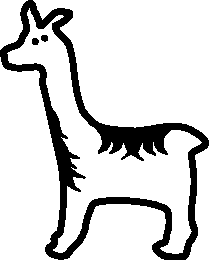
\includegraphics[height=1in]{llama.pdf}
\end{center}

Lable the measure of your triangles angles as $\alpha$, $\beta$, and
$\gamma$. We would like to parade Louie around the triangle.
\begin{enumerate}
\item Through what angle does Louie rotate when he strolls around a
  vertex?
\item How many degrees did the ``cut'' rotate Louie? 
\end{enumerate}

\end{question}

\mynewpage


\begin{question}
If a cone is made on a sheet of paper with a cut of $\theta$ degrees,
and a triangle is made surrounding the point of the cone, what is the
sum of the degrees of this triangle?
\end{question}



\end{document}
